\documentclass[12pt,a4paper]{article}
\usepackage[utf8]{inputenc}
\usepackage{amsmath}
\usepackage{amsfonts}
\usepackage{amssymb}
\usepackage{makeidx}
\usepackage{graphicx}
\usepackage{lmodern}
\usepackage{url}
\usepackage{bm}
\usepackage{booktabs}
\usepackage{float}
\usepackage[left=2cm,right=2cm,top=2cm,bottom=2cm]{geometry}
\author{Mudathir Mahgoub}
\title{Project report}
\begin{document}

\maketitle

\section{Description of PDL solver}
This PDL solver checks the satisfiability of formulas in propositional dynamic logic (PDL).
The input is a kripke frame, which is optional, followed by a formula in PDL. The output is the satisfiability result of this formula which is either \textit{unsat}, \textit{sat} or \textit{unknown}. If the result is \textit{sat}, the solver outputs a kripke frame that satisfies the formula. Furthermore, it specifies the set of states where the formula is satisfied. If this set is equal to $K$, the set of all states in the kripke frame, then the formula is valid in this kripke frame. Otherwise, this set satisfies the formula and its complement, with respect to $K$, falsifies the formula. 

To check the validity of a formula in all kripke frames, its negation should be used as an input and if the result is \textit{unsat}, then it is valid. If the result is \textit{sat}, then the returned kripke frame is a counter example that falsifies the original formula.

\section{PDL Complexity}

The satisfiability problem for PDL formulas is decidable, and it is \textit{EXPTIME-complete} (theorm 8.5 in \cite{dynamic}). Therefore the solver may fail to determine the satisfiability within the time limit (by default it is 30 seconds), and hence it returns \textit{unknown} result. 

% THEOREM 6.5 ( SMALL MODEL THEOREM): Let $\varphi$ be a satisfiable formula of
% PDL. Then $\varphi$ is satisfied in a Kripke frame with no more than $2^{\vert \varphi \vert}$ % states.

On the other hand the satisfiability of a PDL formula in a given Kripke frame can be determined in polynomial time (exercise 6.4 in \cite{dynamic}). So one expects this to be easy for CVC4 when the model (Kripke frame) is given and ``check-sat" is executed. Unfortunately, CVC4 doesn't terminate if the formula is \textit{unsat} and uses transitive closure operation. After asking an expert (Andrew Reynolds), apparently CVC4 keeps  ``adding a repeating pattern of lemmas related to transitive closure" which needs to be reviewed. Fortunately I found a work around by just removing the constraint related to the PDL formula and asserting only the frame constraints. After CVC4 finds the model, the PDL formula is evaluated. If the result is true, then it is \textit{sat}, otherwise it is \textit{unsat}.


\subsection{Exercise 6.4}

 The following is my reasoning for this exercise where $K$ is the set of all states in the frame:
\begin{itemize}
\item Formulas $\textbf{0}$, $\textbf{1}$, and atomic propositions are subsets of $K$, therefore they can be computed in $O(\vert K \vert)$.
\item Programs $\textbf{skip}?$, $\textbf{fail}?$, and atomic programs are subsets of $K \times K$, therefore the can be computed in $O(\vert K \vert^2)$.

\item Boolean operators $\neg, \wedge, \vee, \rightarrow, \leftrightarrow$ involves set operations $-, \cap, \cup: \mathbb{P}(K) \times \mathbb{P}(K) \rightarrow \mathbb{P}(K)$ which can be computed in $O(\vert K \vert^2)$ ($O(\vert K \vert)$ if hash tables are used).

\item Program operators $;, \cup, *$ and modal operators $[], \langle \rangle$ involves set operations and relation operations $\circ, *: \mathbb{P}(K \times K) \times \mathbb{P}(K \times K) \rightarrow \mathbb{P}(K \times K)$. Both $\circ$ and $*$ can be computed using graph data structures and DFS algorithm. 
For $\circ$ operation, the DFS algorithm stops at depth 2, and for $*$ it continues until the end. 
If the graph is dense, both operations $\circ, *$ require maximum $O(\vert K \vert^3)$ to be computed for all states (all graph vertices). 

\item If the number of operators in a given formula $\varphi$ is $n$, then the formula semantics $m(\varphi)$ can be evaluated in $O(n \vert K \vert ^3)$. Finally it takes constant time to evaluate $m(\varphi) \neq \varphi$   determine the satisfiability answer. 
\end{itemize}

From the above discussion, the worst case scenario takes $O(n \vert K \vert ^3)$ time which is polynomial. 

\section{Installation}

The following commands download the source code from github and compile it to generate the solver file ``pdl.jar". 

\begin{verbatim}
git clone https://github.com/mudathirmahgoub/pdl
cd pdl
chmod 777 gradlew
./gradlew build
cd bin
chmod 777 cvc4_linux
java -jar pdl.jar -i test.pdl 
java -jar plantuml.jar test.dot
\end{verbatim}



\section{Project components}

The project is primarily code and would use the SMT solver CVC4 as a back end and apply the relation theory to implement the semantics of PDL. The project would import CVC4 abstract syntax tree (AST) for relations from another project that I am working on (Alloy2SMT translator\footnote{\url{https://github.com/CVC4/org.alloytools.alloy/tree/cvc4/alloy2smt}}) which supports type checking and SMT models parsing, albeit it needs some refactoring to be more generic.  For this project I would write a translator from PDL AST to CVC4 AST and display back the SMT models returned from CVC4 as Kripke frames and dot files for visualization using software like graphvis.

Since CVC4 AST is written in Java, I am using Java for this project along with  gradle\footnote{\url{https://github.com/mudathirmahgoub/pdl}}. I have written an ANTLR4 grammar for PDL following the syntax in chapter 5 in \cite{dynamic}. The grammar also handles a kripke frame written using the set notation in chapter 5 with one difference ($m_{\mathfrak{K}}(a)$ would be written as $m(a)$). Lastly I  prepared classes for PDL AST for Kripke frames, formulas and programs. Next tasks would be parsing PDL input into PDL AST and translating this AST into CVC4 AST. 


\section{PDL formula translation}

What does it mean to have a satisfiable formula in PDL ?

A PDL formula $\varphi$ is satisfiable if there exists a kripke frame $\mathfrak{K}=(K, m_{\mathfrak{K}})$ and a state  $u$ such that $u \in m_{\mathfrak{K}}(\varphi) $, and we write $\mathfrak{K}, u \models \varphi$. In simple words, a formula is satisfiable if its meaning is nonempty in some kripke frame (i.e. $m_{\mathfrak{K}}(\varphi) \neq \phi$). 

Since the PDL semantics uses set and relation operations, they are translated directly into their corresponding operations in the relation theory in CVC4. The only exception is the reflexive transitive closure $*$ which is not supported directly in CVC4, but supported through the built-in transitive closure. Table \ref{tab:translation} summarizes this translation. Other PDL operators are defined using the basic operators in table \ref{tab:translation}. 

\begin{table}
\begin{center}
\begin{tabular}{ll} 
\toprule
PDL & CVC4 \\    
\midrule    
$K=\lbrace u_0, u_1, \cdots u_n \rbrace$ &  
$\begin{matrix}
\text{\textbf{Atom} : \text{Uninterpreted sort}} \\
u_0, u_1, \cdots, u_n: \textbf{Atom} \\
\textit{atomUniverse}: \text{Set(Tuple (\textbf{Atom}))} = \lbrace \langle u_0 \rangle, \langle u_1 \rangle, \cdots , \langle u_n \rangle \rbrace \\
\textit{atomIdentity}:  = \lbrace \langle u_0, u_0 \rangle, \langle u_1, u_1 \rangle, \cdots , \langle u_n, u_n \rangle \rbrace \\
\end{matrix}$ \\ \midrule   
\textbf{0} & \textit{emptyset} : (Set (Tuple \textbf{Atom})) \\
\textbf{1} & \textit{atomUniverse} \\
Atomic propositions $p, q, r, \cdots$ & $p, q, r, \cdots : \text{Set(Tuple (\textbf{Atom}))}$ \\
Atomic programs $a, b, c, \cdots$ & $a, b, c \cdots : \text{Set(Tuple (\textbf{Atom}$\times$\textbf{Atom}))}$ \\
$p \vee q$ & $p \cup q$ \\
$p \wedge q$ & $p \cap q$ \\
$\neg p$ & $\textit{atomUniverse} - p$ \\
$p \rightarrow q$ & $(\textit{atomUniverse}- p)\cup q$ \\
$a;b$ & $a \circ b$ where $\circ$ is the join operator\\
$a;b$ & $a \circ b$ where $\circ$ is the join operator\\
$a \cup b$ (choice) & $a \cup b$ (union)\\
$a*$ (choice) & $a \cup a^+$  where $a^+$ is the transitive closure of $a$\\
$p?$ (test) & $(p \times p) \cup \textit{atomIdentity}$ where $\times$ is the cross product\\
\bottomrule
\end{tabular}
\end{center}
\caption{PDL translation to CVC4} \label{tab:translation}
\end{table}

What does is the meaning of the operator $\leftrightarrow$

\section{Examples}

\subsection{A PDL formula without Kripke frame}

\subsubsection*{Input}
\begin{verbatim}
(p and q) and
<do p -> a | q -> b od>
    (
        (<b> (p and not q))  and
        (<a> (q and not p))
    )
\end{verbatim}
The above formula is equivalent to:
\begin{align*}
((p \wedge q) \wedge \langle\textbf{ do }p \rightarrow a \vert q \rightarrow b\textbf{ od }\rangle(\langle b\rangle(p \wedge \neg q) \wedge \langle a \rangle(q \wedge \neg p)))
\end{align*}
\subsection*{Output (.kripke file)}
\begin{verbatim}
K = {0, 2, 1, 3}
m(p) = {0, 3}
m(q) = {1, 3}
m(a) = {(2,1), (3,2)}
m(b) = {(2,0)}
Satisfying states: [3]
\end{verbatim}
\subsection*{Output (.dot file)}

\begin{figure}[H]
\center
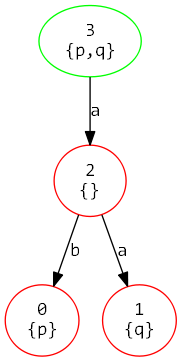
\includegraphics[scale=0.4]{example1.png}

\caption{The formula is satisfied in state $3$ (green) and unsatisfied in states $0, 1, 2$ (red). }
\end{figure}


\subsection{A PDL formula with Kripke frame}

\subsubsection*{Input}
\begin{verbatim}
K = {01,2,3,4,5}
m(p) = {01,2,4}
m(q) = {01, 3}
m(r) = {5}
m(a) = {(01,2), (01,4), (2,4), (01,3)}
m(b) = {(01,3), (3,3)}
m(c) = {(5,5)}
[a union b union c] (q and not p)
\end{verbatim}
The above formula is equivalent to:
\begin{align*}
[((a \cup b) \cup c)](q \wedge \neg p)
\end{align*}
\subsection*{Output (.kripke file)}
\begin{verbatim}
K = {s01, s2, s3, s4, s5}
m(p) = {s01, s2, s4}
m(q) = {s01, s3}
m(r) = {s5}
m(a) = {(s01,s2), (s01,s4), (s2,s4), (s01,s3)}
m(b) = {(s01,s3), (s3,s3)}
m(c) = {(s5,s5)}
Satisfying states: [s3, s4]
\end{verbatim}
\subsection*{Output (.dot file)}

\begin{figure}[H]
\center
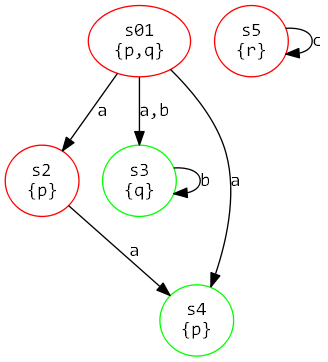
\includegraphics[scale=0.4]{example2.png}

\caption{The formula is satisfied in states $s3, s4$ (green) and unsatisfied in states $s01, s2, s5$ (red). }
\end{figure}



\bibliographystyle{plain}

\bibliography{references}

\end{document}
